\documentclass[10pt]{article}
\usepackage[pdftex]{graphicx}
\usepackage{epstopdf}
\usepackage[utf8x]{inputenc}

%-----------------------------------------------------------------------------%
% Margins:
%-----------------------------------------------------------------------------%

\special{papersize=8.5in,11in} \setlength{\topmargin}{0in}
\setlength{\headheight}{0in} \setlength{\headsep}{0in}
\setlength{\textheight}{8.75in} \setlength{\oddsidemargin}{0in}
\setlength{\textwidth}{6.5in}

%-----------------------------------------------------------------------------%
% Font:
%-----------------------------------------------------------------------------%

\usepackage[T1]{fontenc}
\usepackage{textcomp}
\usepackage{palatino}
\usepackage{mathpazo}
\usepackage{stmaryrd}
%\usepackage{dsfont}

%-----------------------------------------------------------------------------%
% PDF:
%-----------------------------------------------------------------------------%

\usepackage{hyperref}
\hypersetup{pdfpagemode=UseNone}
\usepackage[all]{hypcap}

%-----------------------------------------------------------------------------%
% Various packages:
%-----------------------------------------------------------------------------%

\usepackage{amsfonts}
\usepackage{amssymb}
\usepackage{amsmath}
\usepackage{latexsym}
\usepackage{amsthm}
\usepackage{eepic}
\usepackage{epsfig}
\usepackage{epstopdf}
\usepackage{sectsty}
\usepackage{graphicx}
\usepackage[usenames]{color}

%-----------------------------------------------------------------------------%
% Theorem-like environments:
%-----------------------------------------------------------------------------%

\newtheorem{theorem}{Theorem}
\newtheorem{lemma}[theorem]{Lemma}
\newtheorem{prop}[theorem]{Proposition}
\newtheorem{cor}[theorem]{Corollary}
\theoremstyle{definition}
\newtheorem{definition}[theorem]{Definition}
\newtheorem{claim}[theorem]{Claim}
\newtheorem{problem}[theorem]{Problem}
\newtheorem{remark}[theorem]{Remark}
\newtheorem*{fact}{Fact}
\newtheorem{example}[theorem]{Example}
\newtheorem{corollary}{Corollary}

%-----------------------------------------------------------------------------%
% Macros:
%-----------------------------------------------------------------------------%

\newcommand{\comment}[1]{\begin{quote}\sf [*** #1 ***]\end{quote}}
\newcommand{\tinyspace}{\mspace{1mu}}
\newcommand{\microspace}{\mspace{0.5mu}}
\newcommand{\op}[1]{\operatorname{#1}}

\newcommand{\norm}[1]{\left\lVert\tinyspace#1\tinyspace\right\rVert}
\newcommand{\snorm}[1]{\lVert\tinyspace#1\tinyspace\rVert}
\newcommand{\abs}[1]{\left\lvert\tinyspace #1 \tinyspace\right\rvert}
\newcommand{\ceil}[1]{\left\lceil #1 \right\rceil}
\newcommand{\floor}[1]{\left\lfloor #1 \right\rfloor}
\def\iso{\cong}
\newcommand{\defeq}{\stackrel{\smash{\text{\tiny def}}}{=}}
\newcommand{\tr}{\operatorname{Tr}}
\newcommand{\rank}{\operatorname{rank}}
\renewcommand{\det}{\operatorname{Det}}
\renewcommand{\vec}{\operatorname{vec}}
\newcommand{\im}{\operatorname{Im}}
\renewcommand{\t}{{\scriptscriptstyle\mathsf{T}}}
\newcommand{\ip}[2]{\left\langle #1 , #2\right\rangle}
\newcommand{\sip}[2]{\langle #1 , #2\rangle}
\def\({\left(}
\def\){\right)}
\def\I{\mathbb{1}}

\newcommand{\triplenorm}[1]{%
  \left|\!\microspace\left|\!\microspace\left| #1
  \right|\!\microspace\right|\!\microspace\right|}

\newcommand{\fid}{\operatorname{F}}
\newcommand{\setft}[1]{\mathrm{#1}}
\newcommand{\lin}[1]{\setft{L}\left(#1\right)}
\newcommand{\density}[1]{\setft{D}\left(#1\right)}
\newcommand{\unitary}[1]{\setft{U}\left(#1\right)}
\newcommand{\trans}[1]{\setft{T}\left(#1\right)}
\newcommand{\herm}[1]{\setft{Herm}\left(#1\right)}
\newcommand{\pos}[1]{\setft{Pos}\left(#1\right)}
\newcommand{\pd}[1]{\setft{Pd}\left(#1\right)}
\newcommand{\sphere}[1]{\mathcal{S}\!\left(#1\right)}
\newcommand{\opset}[3]{\setft{#1}_{#2}\!\left(#3\right)}

\def\complex{\mathbb{C}}
\def\real{\mathbb{R}}
\def\natural{\mathbb{N}}
\def\integer{\mathbb{Z}}

\def \lket {\left|}
\def \rket {\right\rangle}
\def \lbra {\left\langle}
\def \rbra {\right|}
\newcommand{\ket}[1]{\lket\microspace #1 \microspace\rket}
\newcommand{\bra}[1]{\lbra\microspace #1 \microspace\rbra}

\newenvironment{mylist}[1]{\begin{list}{}{
    \setlength{\leftmargin}{#1}
    \setlength{\rightmargin}{0mm}
    \setlength{\labelsep}{2mm}
    \setlength{\labelwidth}{8mm}
    \setlength{\itemsep}{0mm}}}
    {\end{list}}

\newcommand{\class}[1]{\textup{#1}}
\newcommand{\prob}[1]{\textit{#1}}
\newcommand{\reg}[1]{\mathsf{#1}}

\newcommand{\HRule}{\rule{\linewidth}{0.5mm}}

\newenvironment{namedtheorem}[1]
           {\begin{trivlist}\item {\bf #1.}\em}{\end{trivlist}}

\def\X{\mathcal{X}}
\def\Y{\mathcal{Y}}
\def\Z{\mathcal{Z}}
\def\W{\mathcal{W}}
\def\A{\mathcal{A}}
\def\B{\mathcal{B}}
\def\V{\mathcal{V}}
\def\U{\mathcal{U}}
\def\C{\mathcal{C}}
\def\D{\mathcal{D}}
\def\E{\mathcal{E}}
\def\F{\mathcal{F}}
\def\M{\mathcal{M}}
\def\R{\mathcal{R}}
\def\P{\mathcal{P}}
\def\Q{\mathcal{Q}}
\def\S{\mathcal{S}}
\def\T{\mathcal{T}}
\def\K{\mathcal{K}}
\def\H{\mathcal{H}}
\def\yes{\text{yes}}
\def\no{\text{no}}

\usepackage{float}
\floatstyle{ruled}
\newfloat{program}{h}{lop}
\floatname{program}{Listing }

\begin{document}

\begin{titlepage}

\begin{center}


% Upper part of the page

\includegraphics{Figures/Logo.png}\\[1cm]    

\textsc{\LARGE University of Waterloo}\\[1.5cm]

\textsc{\Large Institute for Quantum Computing}\\[0.5cm]


% Title
\HRule \\[0.4cm]
{ \huge \bfseries QCViewer User-Guide}\\[0.4cm]

\HRule \\[1.5cm]

\vfill

% Bottom of the page
{\large \today}
{\large Version 0.8}

\end{center}

\end{titlepage}

\tableofcontents
\newpage

    \begin{flushright}
    QCViewer 0.8 Documentation
    \end{flushright}

%% Introduction
%%%%%%%%%%%%%%%%%%%%%%%%%%%%%%%%%%%%%%%%%%%%%%%%%%%%%%%%%%%%%%
\section{Introduction} \label{sec:Introduction}

QCViewer is a tool for displaying, editing, and simulating quantum circuits. 

\begin{center}
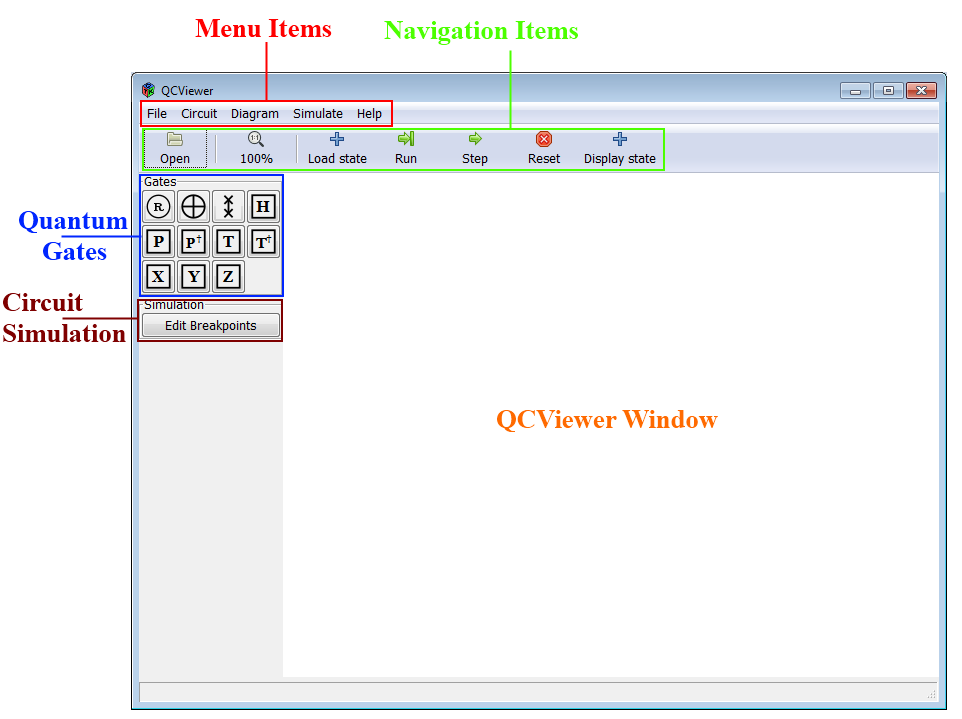
\includegraphics[scale=0.50]{Figures/QCViewerGUI.png} \\
The QCViewer program.
\end{center}

It allows users to test new circuit designs and make publication quality diagrams with an easy to use graphical interface. Supported features also include simulation of the circuit while graphically displaying the current state. The most recent version and changelog can be found \href{http://qcirc.iqc.uwaterloo.ca/index.php?n=Projects.QCViewer}{here}. 

%% Creating a Circuit
%%%%%%%%%%%%%%%%%%%%%%%%%%%%%%%%%%%%%%%%%%%%%%%%%%%%%%%%%%%%%%
\section{Creating a Circuit} \label{sec:CreatingaCircuit}
In this section, we'll go through the creation and execution of a simple circuit to illustrate the functionality of QCViewer. We will be preparing a simple EPR (Einstein-Podolsky-Rosen) circuit as shown below.
\begin{center}
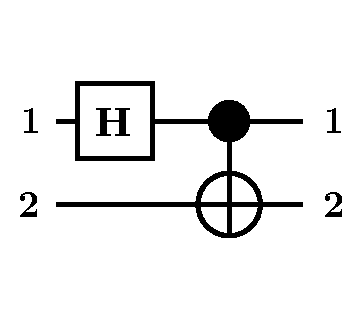
\includegraphics[scale=.7]{Figures/CreateCircuit/EPRCircuit}\\
Circuit for EPR Pair.
\end{center}

From the Circuit menu 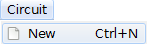
\includegraphics{Figures/CreateCircuit/New.png} select \em New \em. A dialog box asking how many qubits you wish to have in your circuit appears. 

\begin{center}
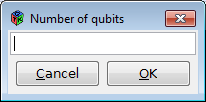
\includegraphics{Figures/CreateCircuit/NumberOfQubits.png}\\
Dialog box asking for number of qubits.
\end{center}

The circuit in this example uses 2 qubits so you may enter ``2'' here. We are then presented with our template circuit.

\begin{center}
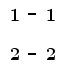
\includegraphics[scale=.7]{Figures/CreateCircuit/TemplateCircuit}\\
Template circuit for 2 qubits.
\end{center}

We may then make use of the gate palette to place the desired gates onto our circuit. In this case we first need a Hadamard gate. Simply click and drag the 
\includegraphics{Figures/Gates/Hadamard.png} graphic onto the template. Next follow this action by placing the 
\includegraphics{Figures/Gates/Mod2.png} graphic to the bottom right of the recently placed Hadamard gate. This should yield a circuit resembling the following

\begin{center}
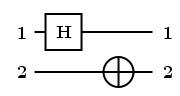
\includegraphics[scale=.7]{Figures/CreateCircuit/EPRCircuit2}
\end{center}

Next, we wish to add a control to complete our CNOT gate on the right. This can be accomplished by simply clicking on the 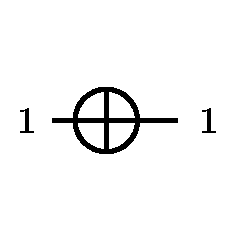
\includegraphics[scale=0.60]{Figures/CreateCircuit/CNOT} in our main cavas. This modifies the menu on the right and adds a \em Properties \em portion. 

\begin{center}
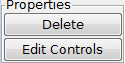
\includegraphics{Figures/CreateCircuit/Properties.png}
\end{center}

By selecting the \em Edit Controls \em option under the \em Properties \em menu, the mouse cursor is changed to 
\includegraphics[scale=0.5]{Figures/CreateCircuit/Cursor.png}. You may now click where you wish to place this control on the circuit. This completes our EPR circuit. 

\subsection{Circuit Simulation}\label{sub:CircuitSimulation}
Now that we have created the circuit, we can simulate the behavior of this circuit given a particular state. Since we are dealing with a circuit consisting of two wires, the dimensionality of our quantum system must abide by this dimensionality as well.

To load a particular quantum state, click the 
\includegraphics[scale=0.60]{Figures/Navigation/LoadState.png} icon to prompt the following dialog box to appear.

\begin{center}
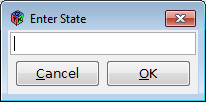
\includegraphics{Figures/CreateCircuit/LoadState.png}
\end{center}

To specify a particular state to enter, the ket formalism is represented by prefixing the state with ``|"  and terminating the state with the less than symbol``>". For instance, if we chose our input state to be $\ket{00}$, this is equivalent to inputting ``|00>". Once we input our state, it is loaded as input into our circuit. By selecting 
\includegraphics[scale=0.60]{Figures/Navigation/DisplayState.png} the state of the qubits are displayed below.

\begin{center}

\includegraphics{Figures/CreateCircuit/DisplayState.png}
\end{center}

In order to observe the progression of our state through the circuit step by step, we manipulate the 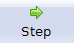
\includegraphics[scale=0.60]{Figures/Navigation/Step.png} button. Using this button highlights the current gate the qubits are interacting with, and display the corresponding states through \em Display State \em. Running the entire course of the circuit can also be done by simply using the 
\includegraphics[scale=0.60]{Figures/Navigation/Run.png} button. By using the reset 
\includegraphics[scale=0.60]{Figures/Navigation/Reset.png} button, one may reset the configuration back to its initial state.

\subsubsection{Example: Grover}

Figure \ref{f:simulate} shows the results of simultating the circuit show in figure \ref{f:groverex} 
(the specification of this circuit can be seen in listing \ref{qc:grover}).  This simulation is done by loading
the state $(H|0\rangle)^{\otimes 5}|1\rangle$.  The first image shows the inital state and the following images 
show the sate after each iteration.

\begin{figure}
\capstart
\centering
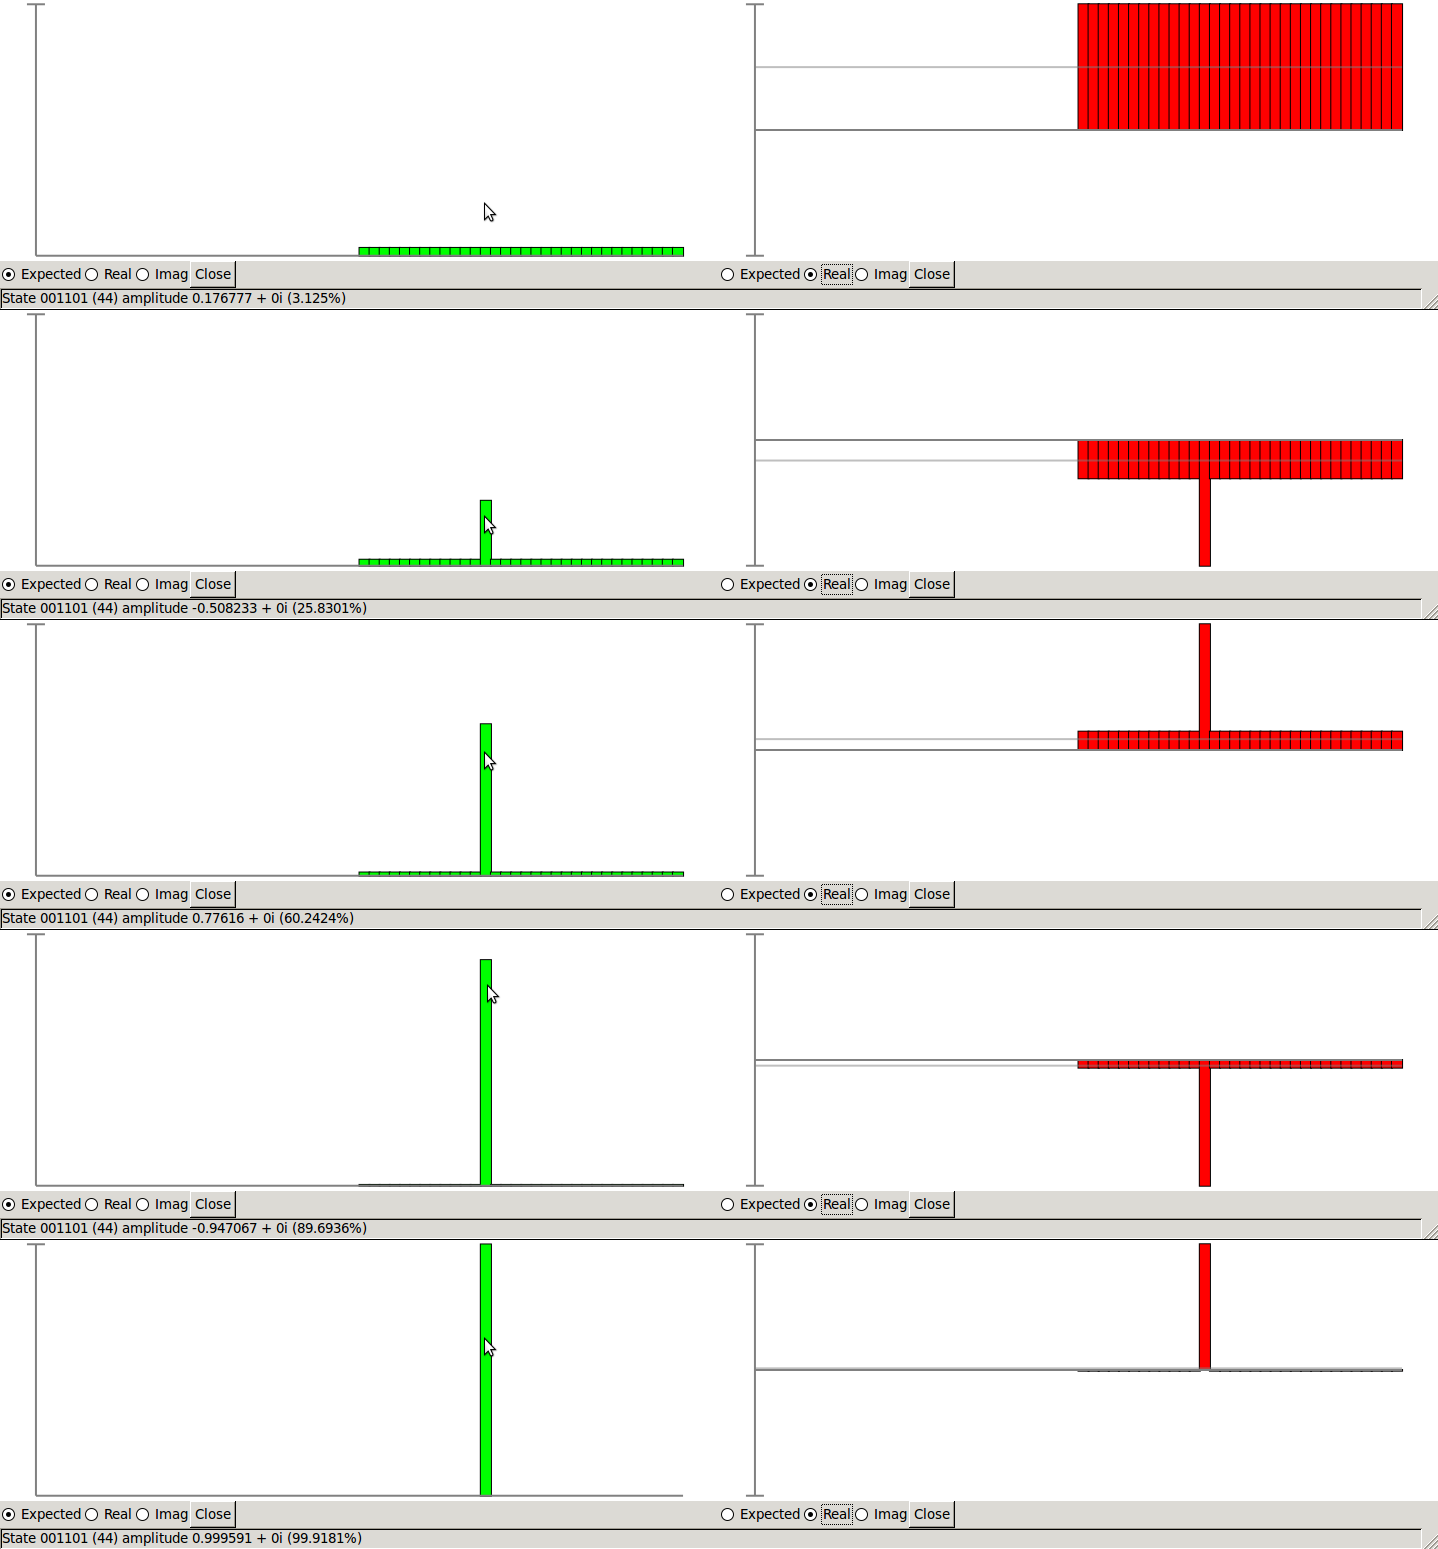
\includegraphics[scale=.35]{Figures/simulate}
\caption{The first row shows the state $(H|0\rangle)^{\otimes 5}|1\rangle$, 
and the subsequent rows show the state as it goes through four iterations of the Grover's iterate. The
diagram for the circuit that generated these pictures can be seen in Figure \ref{f:groverex}.}
\label{f:simulate}
\end{figure}

%% QCViewer Components
%%%%%%%%%%%%%%%%%%%%%%%%%%%%%%%%%%%%%%%%%%%%%%%%%%%%%%%%%%%%%%
\section{QCViewer Components}\label{sec:QCViewerComponents}

%% Quantum Gates
%%%%%%%%%%%%%%%%%%%%%%%%%%%%%%%%%%%%%%%%%%%%%%%%%%%%%%%%%%%%%%
\subsection{Quantum Gates} \label{sub:QuantumGates}

QCViewer provides the user a gate palette that allows one to add various gates to construct a quantum circuit. Each of the gates in the palette can be represented as linear operators or matrices acting upon some quantum system. 

\begin{center}
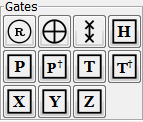
\includegraphics{Figures/Gates/Gates.png}\\
Quantum gate palette
\end{center}

What follows is a more in-depth listing of the provided quantum gates in QCViewer and their corresponding matrix equivalents. 

\begin{itemize}
\item 
\includegraphics{Figures/Gates/RotationGate.png}  Rotation Operator

The rotation gates are exponentiated Pauli matrices that correspond to rotations on the Bloch sphere about the $\hat{x}, \hat{y}$ or $\hat{z}$ axes.

\begin{center}
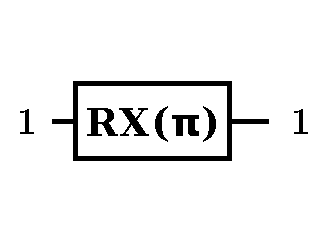
\includegraphics[scale=.7]{Figures/Gates/RotXGateViewer} 
  \begin{minipage}{.9\linewidth}
    \begin{equation*} \label{mat:rotX}
    \renewcommand{\arraystretch}{1.25}
 R_x(\theta) \equiv e^{-i\theta X/2} = \cos\frac{\theta}{2} I - i \sin \frac{\theta}{2} X =  \begin{pmatrix} \cos \frac{\theta}{2} & -i\sin\frac{\theta}{2} \\ -i\sin\frac{\theta}{2} & \cos\frac{\theta}{2}\end{pmatrix}
    \end{equation*}
  \end{minipage}\hspace{-2.5cm}
  \begin{minipage}{.2\linewidth}
  \vspace*{3pt}
    \begin{align}
    \end{align}
  \end{minipage}
\end{center}

\begin{center}
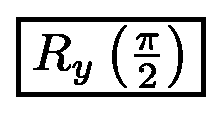
\includegraphics[scale=.7]{Figures/Gates/RotYGateViewer}  
  \begin{minipage}{.9\linewidth}
    \begin{equation*} \label{mat:rotY}
    \renewcommand{\arraystretch}{1.25}
R_y(\theta) \equiv e^{-i\theta Y/2} = \cos\frac{\theta}{2} I - i \sin \frac{\theta}{2} Y =  \begin{pmatrix} \cos \frac{\theta}{2} & -\sin\frac{\theta}{2} \\ \sin\frac{\theta}{2} & \cos\frac{\theta}{2}\end{pmatrix}
    \end{equation*}
  \end{minipage}\hspace{-2.5cm}
  \begin{minipage}{.2\linewidth}
  \vspace*{3pt}
    \begin{align}
    \end{align}
  \end{minipage}
\end{center}

\begin{center}
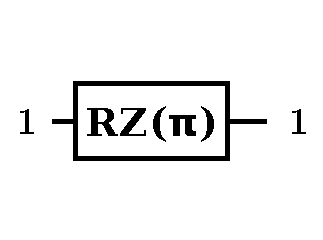
\includegraphics[scale=.7]{Figures/Gates/RotZGateViewer} 
  \begin{minipage}{.9\linewidth}
    \begin{equation*} \label{mat:RotZ}
    \renewcommand{\arraystretch}{1.25}
R_z(\theta) \equiv e^{-i\theta Z/2} = \cos\frac{\theta}{2} I - i \sin \frac{\theta}{2} Z =  \begin{pmatrix} e^{-i\theta/2} & 0 \\ 0 & e^{i \theta/2}\end{pmatrix}
    \end{equation*}
  \end{minipage}\hspace{-2.5cm}
  \begin{minipage}{.2\linewidth}
  \vspace*{3pt}
    \begin{align}
    \end{align}
  \end{minipage}
\end{center}

Selecting which axis to rotate on and modifying the $\theta$ value for these gates can be accomplished in the \em Rotation \em dialog box appearing to the left when manipulating one of these gates.

\begin{center}
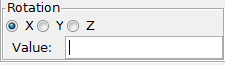
\includegraphics{Figures/Gates/RotationDialog.png}\\
Rotation dialog box.
\end{center}

Putting in a value, $v$ into the dialog box corresponds to $(v)\pi$ along which ever axis is specified by the radio buttons above. 

\item 
\includegraphics{Figures/Gates/Mod2.png}  Addition Modulo Two

The $\oplus$ symbol denotes an addition modulo two operation on two quantum qubits. This is generally denoted as $a \oplus b$ for some qubits $a$ and $b$. 

\item 
\includegraphics{Figures/Gates/SwapGate.png}  Swap Gate

The SWAP gate is capable of swapping two quantum states.

\begin{center}
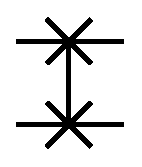
\includegraphics[scale=.7]{Figures/Gates/SwapGateViewer} \\
  \begin{minipage}{.9\linewidth}
    \begin{equation*} \label{mat:Swap}
    \renewcommand{\arraystretch}{1.25}
SWAP = \begin{pmatrix} 1 & 0 & 0 & 0 \\ 0 & 0 & 1 & 0 \\ 0 & 1 & 0 & 0 \\ 0 & 0 & 0 & 1\end{pmatrix}
    \end{equation*}
  \end{minipage}\hspace{-2.5cm}
  \begin{minipage}{.2\linewidth}
  \vspace*{3pt}
    \begin{align}
    \end{align}
  \end{minipage}
\end{center}

\item 
\includegraphics{Figures/Gates/Hadamard.png}  Hadamard Gate

The Hadamard gate acts on a single qubit and maps the basis state $\ket{0}$ to $\frac{1}{\sqrt 2}(\ket{0} + \ket{1})$ and basis state $\ket{1}$ to $\frac{1}{\sqrt 2}(\ket{0} - \ket{1})$. 

\begin{center}
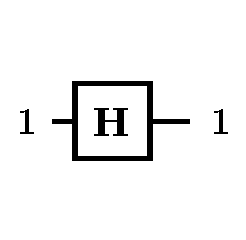
\includegraphics[scale=.7]{Figures/Gates/HadamardViewer} \\
  \begin{minipage}{.9\linewidth}
    \begin{equation*} \label{mat:Hadamard}
    \renewcommand{\arraystretch}{1.25}
H =  \frac{1}{\sqrt 2}\begin{pmatrix} 1 & 1 \\ 1 & \textnormal{-}1 \end{pmatrix}
    \end{equation*}
  \end{minipage}\hspace{-2.5cm}
  \begin{minipage}{.2\linewidth}
  \vspace*{3pt}
    \begin{align}
    \end{align}
  \end{minipage}
\end{center}

\item 
\includegraphics{Figures/Gates/PGate.png} 

\begin{center}

\includegraphics[scale=.7]{Figures/Gates/PGateViewer} \\

\begin{minipage}{.9\linewidth}
    \begin{equation*} \label{mat:PGate}
    \renewcommand{\arraystretch}{1.25}
P = \begin{pmatrix} 1 & 0 \\ 0 & i \end{pmatrix}
    \end{equation*}
  \end{minipage}\hspace{-2.5cm}
  \begin{minipage}{.2\linewidth}
  \vspace*{3pt}
    \begin{align}
    \end{align}
  \end{minipage}
\end{center}

\item 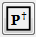
\includegraphics{Figures/Gates/PAdjointGate.png} 

\begin{center}
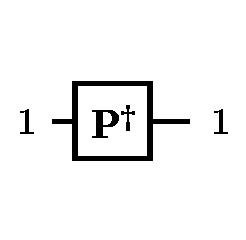
\includegraphics[scale=.7]{Figures/Gates/PAdjointGateViewer} \\
\begin{minipage}{.9\linewidth}
    \begin{equation*} \label{mat:PGateAdjoint}
    \renewcommand{\arraystretch}{1.25}
P^\dagger = \begin{pmatrix} 1 & 0 \\ 0 & -i \end{pmatrix}
    \end{equation*}
  \end{minipage}\hspace{-2.5cm}
  \begin{minipage}{.2\linewidth}
  \vspace*{3pt}
    \begin{align}
    \end{align}
  \end{minipage}
\end{center}

\item 
\includegraphics{Figures/Gates/TGate.png}  $\frac{\pi}{8}$ Gate

\begin{center}

\includegraphics[scale=.7]{Figures/Gates/TGateViewer} \\

  \begin{minipage}{.9\linewidth}
    \begin{equation*} \label{mat:TGate}
    \renewcommand{\arraystretch}{1.25}
T = e^{i \pi/8}\begin{pmatrix} e^{-i\pi/8} & 0 \\ 0 & e^{i\pi/8} \end{pmatrix}
    \end{equation*}
  \end{minipage}\hspace{-2.5cm}
  \begin{minipage}{.2\linewidth}
  \vspace*{3pt}
    \begin{align}
    \end{align}
  \end{minipage}
\end{center}

\item 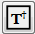
\includegraphics{Figures/Gates/TAdjointGate.png} 

\begin{center}
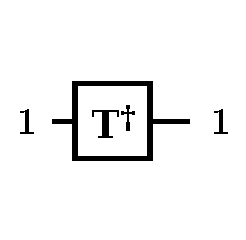
\includegraphics[scale=.7]{Figures/Gates/TAdjointGateViewer} \\

\begin{minipage}{.9\linewidth}
    \begin{equation*} \label{mat:TGateAjoint}
    \renewcommand{\arraystretch}{1.25}
T^\dagger = e^{i \pi/8}\begin{pmatrix} e^{i\pi/8} & 0 \\ 0 & e^{-i\pi/8} \end{pmatrix}
    \end{equation*}
  \end{minipage}\hspace{-2.5cm}
  \begin{minipage}{.2\linewidth}
  \vspace*{3pt}
    \begin{align}
    \end{align}
  \end{minipage}

\end{center}

\item 
\includegraphics{Figures/Gates/XGate.png}  Pauli-X Gate

The Pauli-X Gate acts on a single qubits and corresponds to a rotation around the X-axis of the Bloch sphere by $\pi$ radians.

\begin{center}

\includegraphics[scale=.7]{Figures/Gates/XGateViewer} \\
  \begin{minipage}{.9\linewidth}
    \begin{equation*} \label{mat:XGate}
    \renewcommand{\arraystretch}{1.25}
X = \begin{pmatrix} 0 & 1 \\ 1 & 0 \end{pmatrix}
    \end{equation*}
  \end{minipage}\hspace{-2.5cm}
  \begin{minipage}{.2\linewidth}
  \vspace*{3pt}
    \begin{align}
    \end{align}
  \end{minipage}
\end{center}

The Pauli-X Gate is essentially the quantum NOT as it maps the qubit states $\ket{0}$ to $\ket{1}$ and $\ket{1}$ to $\ket{0}$. 

\item 
\includegraphics{Figures/Gates/YGate.png}  Pauli-Y Gate

The Pauli-Y Gate acts on a single qubit and corresponds to a rotation about the Y-axis of the Bloch sphere by $\pi$ radians. The matrix representation of this gate is provided below. 

\begin{center}
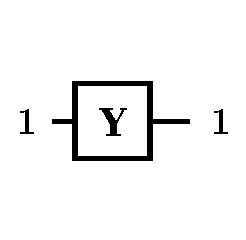
\includegraphics[scale=.7]{Figures/Gates/YGateViewer} \\
  \begin{minipage}{.9\linewidth}
    \begin{equation*} \label{mat:YGate}
    \renewcommand{\arraystretch}{1.25}
Y = \begin{pmatrix} 0 & \textnormal{-}i \\ i & 0 \end{pmatrix}
    \end{equation*}
  \end{minipage}\hspace{-2.5cm}
  \begin{minipage}{.2\linewidth}
  \vspace*{3pt}
    \begin{align}
    \end{align}
  \end{minipage}
\end{center}

It maps the basis states $\ket{0}$ to $i\ket{1}$ and $\ket{1}$ to $-i\ket{0}$. 

\item 
\includegraphics{Figures/Gates/ZGate.png}  Pauli-Z Gate

The Pauli-Z Gate acts on a single qubit and corresponds to a rotation about the Z-axis of the Bloch sphere by $\pi$ radians. The matrix representation of this gate is provided below.

\begin{center}

\includegraphics[scale=.7]{Figures/Gates/ZGateViewer} \\
  \begin{minipage}{.9\linewidth}
    \begin{equation*} \label{mat:ZGate}
    \renewcommand{\arraystretch}{1.25}
Z = \begin{pmatrix} 1 & 0 \\ 0 & \textnormal{-}1 \end{pmatrix}
    \end{equation*}
  \end{minipage}\hspace{-2.5cm}
  \begin{minipage}{.2\linewidth}
  \vspace*{3pt}
    \begin{align}
    \end{align}
  \end{minipage}
\end{center}

It maps the basis states $\ket{0}$ to an unchanged $\ket{0}$ and maps $\ket{1}$ to $-\ket{1}$. 

\end{itemize}

%% Navigation Bar
%%%%%%%%%%%%%%%%%%%%%%%%%%%%%%%%%%%%%%%%%%%%%%%%%%%%%%%%%%%%%%
\subsection{Navigation Bar}\label{sub:NavigationBar}

\begin{center}

\includegraphics{Figures/Navigation/NavigationBar.png}
\end{center}

\begin{itemize}
\item 
\includegraphics{Figures/Navigation/Open.png} \\ 

Clicking the \em Open \em icon prompts a dialog box to appear that allows the user to select previously saved circuits as .qc files to open.

\begin{center}
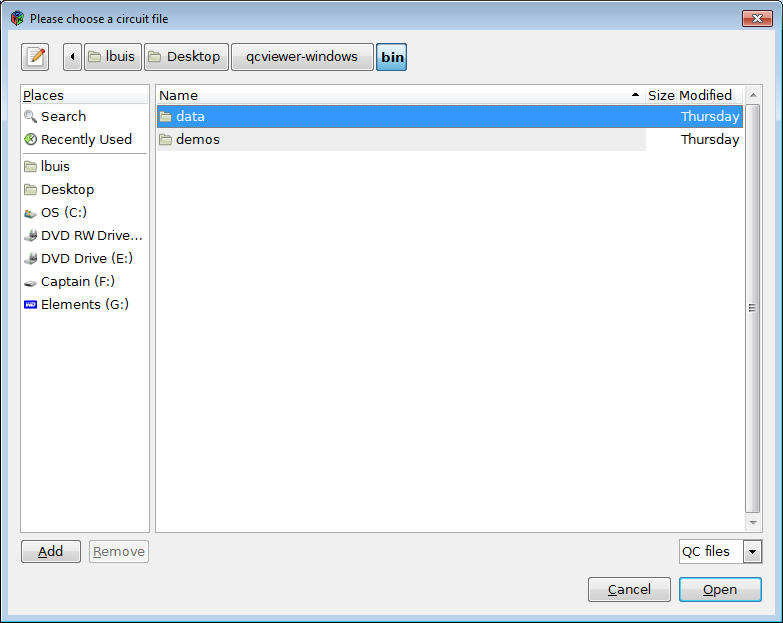
\includegraphics[scale=0.75]{Figures/Navigation/OpenDialog.png}
\end{center}

If no circuits have been previously saved by the user, QCViewer does come with a number of demo circuits in the ``demos" folder. 

\item 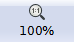
\includegraphics{Figures/Navigation/Ratio.png}\\ 

Depending on the number of elements in the QCViewer window, clicking this graphic provides a 1:1 perspective on what exists in the window. For instance if you zoom too far in or out (via the mouse scroll wheel), then clicking this will bring you back to viewing the contents in a 1:1 ratio. 

\item 
\includegraphics{Figures/Navigation/LoadState.png} \\ 

This button allows one to load a quantum state into the circuit currently in QCViewer. The quantum state must be of proper dimensionality, that is, equal to the dimensionality of the circuit. Clicking this graphic prompts a dialog box to ask for the user to enter the state. 

\begin{center}
\includegraphics{Figures/Navigation/LoadStateDialog.png}
\end{center}

Input states must take the form of 

\begin{eqnarray}
``| \underbrace{b \dots b}_n >"  
\end{eqnarray}

where $b \in \{0,1\}$ and $n$ is the dimensionality of the circuit and the quotation marks are just for clarity.

\item \includegraphics{Figures/Navigation/Run.png}\\

The \em Run \em icon allows the associated quantum state of a circuit to run its entire course. For a specific example use of the \em Run \em functionality, refer to Section~\ref{sec:CreatingaCircuit}

\item \includegraphics{Figures/Navigation/Step.png}\\

The \em Step \em icon allows the user to step through each time step individually. For a specific example use of the \em Step \em functionality, refer to Section~\ref{sec:CreatingaCircuit}

\item \includegraphics{Figures/Navigation/Reset.png}\\ 

The \em Reset \em icon allows the user to reset the quantum state associated with the circuit back to the beginning of the circuit. For a specific example use of the \em Reset \em functionality, refer to Section~\ref{sec:CreatingaCircuit}

\item \includegraphics{Figures/Navigation/DisplayState.png} \\

The \em Display State \em item allows the user to visualize the simulation of qubits via traversal of the circuit. Clicking the button yields the following at the bottom portion of QCViewer.

\begin{center}
\includegraphics[scale=0.75]{Figures/DisplayState.png}
\end{center}

For a specific example use of the \em Display State \em functionality, refer to Section~\ref{sec:CreatingaCircuit}

\end{itemize}

%% Menu Bar
%%%%%%%%%%%%%%%%%%%%%%%%%%%%%%%%%%%%%%%%%%%%%%%%%%%%%%%%%%%%%%
\subsection{Menu Bar}\label{sub:MenuBar}

\begin{center}
\includegraphics{Figures/Menu/MenuBar.png}
\end{center}

\begin{itemize}
\item \includegraphics{Figures/Menu/File.png} \\ \\
The {\bf File} menu allows one to quit the QCViewer program.

\item \includegraphics{Figures/Menu/Circuit.png} \\ \\
The {\bf Circuit} menu provides us with the option to create a \em New \em circuit (more information on how to create a circuit refer to  Section~\ref{sec:CreatingaCircuit}. From here, we may also \em Open \em previously saved circuits and \em Save \em the current workspace circuit as a .qc file. The \em Open \em dialog is provided in more detail in Section~\ref{sub:NavigationBar}.

\item \includegraphics{Figures/Menu/Diagram.png} \\ \\ 
The {\bf Diagram} menu option allows one to save the current circuit in the workspace for publication quality circuit diagrams as either png, SVG, or Postscript format. From this menu there are options to \em Show parallel guides \em and \em Show warnings \em, both of which are covered in more detail in Section~\ref{sec:CreatingaCircuit}.
 
\item \includegraphics{Figures/Menu/Simulate.png} \\ \\
The {\bf Simulate} menu harbors the \em Display State \em option which is gone over in greater detail in both Sections~\ref{sub:NavigationBar} and~\ref{sec:CreatingaCircuit}


\item \includegraphics{Figures/Menu/Help.png} \\ \\
The {\bf Help} menu provides additional information about the creators of QCViewer. 

\end{itemize}

%% Working with .qc Files
%%%%%%%%%%%%%%%%%%%%%%%%%%%%%%%%%%%%%%%%%%%%%%%%%%%%%%%%
\section{Working with .qc Files}\label{sec:QCFiles}

When you create a circuit in QCViewer, a corresponding .qc file is generated when the circuit is saved. This file serves as a textual representation of what the circuit consists of. 

\subsection{The Basics of .qc Files}\label{sec:BasicsOfQCFiles}

As an example, given our EPR circuit used in the previous sections:

\begin{center}
\includegraphics[scale=.7]{Figures/QCFiles/EPRCircuit} \\
EPR circuit generated from QCViewer.
\end{center}

The output of the .qc file associated with this circuit is shown in listing \ref{qc:epr}.

\begin{program}
\caption{.qc file generated for epr circuit}
\label{qc:epr}
\begin{verbatim}
.v 1 2
.i 1 2
.o 1 2
.ol 1 2
.c
BEGIN
H 1
tof 1 2
END
\end{verbatim}
\end{program}

The header information consists of the following content:

\begin{itemize}
\item .v: Defines names of the circuit qubits.
\item .i: Specifies which qubits accept primary inputs.
\item .o: Reports primary outputs.
\item .ol: Allows one to alternate names to be specified for the output labels. (Optional parameter).
\item .c: Specifies the values of input constants. (Optional parameter).
\end{itemize}

The primary circuit is represented between BEGIN and END tags. The circuit name is represented as the leftmost string in each line. In the case above, H refers the Hadamard gate and tof refers to the Toffoli gate. The numbers following the names refer to the line of the circuit that the gate resides on. For instance there is a 1 next to the H indicating that the Hadamard gate is on the first line. In the case where there is more than one number as with the Toffoli gate, the rightmost number refers to the line of the circuit that the gate is on, and the rest of the numbers refer to the lines of the circuit that any controls are on.

\subsection{Labeling Circuits}\label{sec:LabelingCircuits}

One may wish to provide labels to the circuit wires and to the collection of gates for succinctness. For example, we may modify the names of the circuit wires and circuit name of the EPR circuit by modifying the respective .qc file as shown in listing \ref{qc:eprl}.

\begin{program}
\caption{ .qc file generated for labeled epr circuit}
\label{qc:eprl}
\begin{verbatim}
.v a b
.i a b
.o a b
.ol a b
.c
BEGIN EPR(a b)
H a
tof a b
END EPR

BEGIN
EPR a b
END
\end{verbatim}
\end{program}

When opening this file in QCViewer, we can see that the wire labels are now a and b opposed to the previous 1 and 2 respectively. We've also provided a name for the circuit (EPR) and refer to this circuit between the main BEGIN and END tags. The respective output from QCViewer is displayed as:

\begin{center}
\includegraphics[scale=.7]{Figures/QCFiles/EPRCircuitLabel} \\
The modified and labeled EPR circuit.
\end{center}

In the next section, we will consider how sub-circuits behave in QCViewer.

%% Sub-Circuits
%%%%%%%%%%%%%%%%%%%%%%%%%%%%%%%%%%%%%%%%%%%%%%%%%%%%%%%%%%%%%%
\section{Sub-Circuits}\label{sec:SubCircuits}

It is often convenient to group gates with a specific functionality together as a sub-circuit for the main circuit. In the \em demos \em folder provided with your distribution of QCViewer there exists a number of demo circuits to try and view. The attention of this section will be focused on the \em grover.qc \em file provided in this distribution (See listing \ref{qc:grover}).

\begin{program}
\caption{ .qc file for the grover circuit}
\label{qc:grover}
\begin{verbatim}
.v a b c d e Workspace
.i a b c d e Workspace
.o a b c d e
.c
BEGIN H5(a b c d e)
H a
H b
H c
H d
H e
END H5

BEGIN GroverIterate (a b c d e Workspace)
H Workspace
T5 a' b' c d e' Workspace
H Workspace

H5 a b c d e

X e
Z a' b' c' d' e
X e

H5 a b c d e
END GroverIterate

BEGIN
H5 a b c d e

GroverIterate^4 a b c d e Workspace 
END

\end{verbatim}
\end{program}

This circuit consists of two sub-circuits labeled H5 and GroverIterate. They are called between the primary BEGIN and END tags to display the following output in figure \ref{f:grover}.

\begin{figure}
\capstart
\centering
\includegraphics[scale=.5]{Figures/SubCircuits/GroverCircuit}
\caption{Grover circuit}
\label{f:grover}
\end{figure}

You can see that these sub-circuits consist of the labels provided in the .qc file. If we wished to expand one of the subcircuits to view the inner content, we may click on the sub-circuit of choice which brings up the subcircuit menu.

\begin{center}
\includegraphics{Figures/SubCircuits/SubCircuitMenu.png} \\
The sub-circuit menu that allows expanding and unrolling the inner content.
\end{center}

\subsection{Expanding Sub-Circuits}\label{sec:ExpandingSubCircuits}

By clicking the \em Expand \em button on the \em Subcircuit \em menu, we see the expanded subcircuit in figure \ref{f:groverex}.

\begin{figure}
\capstart
\centering
\includegraphics[scale=.5]{Figures/SubCircuits/GroverCircuitExpand}
\caption{Grover's circuit expanded.}
\label{f:groverex}
\end{figure}

The subcircuit can similarly be collapsed by clicking the same button afterward.


\subsection{Unrolling Sub-Circuits}\label{sec:UnrollingSubCircuits}

For circuits that have a looping component (covered in greater detail in section~\ref{sec:Miscellaneous}) we may unroll the iterations of the loop using the \em Unroll \em button in the \em Subcircuit \em menu. As we can see from figure \ref{f:groverex}, the Grover Iterate is to repeat 4 times. Unrolling the loop, we are able to view the circuit in its entirety (figure \ref{f:groverunroll}).

\begin{figure}
\capstart
\centering
\includegraphics[width=170mm]{Figures/SubCircuits/GroverCircuitUnroll}
\caption{Grover's circuit unrolled.}
\label{f:groverunroll}
\end{figure}

Similarly, by pressing the \em Unroll \em button afterward, the circuit is collapsed to its previous state. 

%% Miscellaneous
%%%%%%%%%%%%%%%%%%%%%%%%%%%%%%%%%%%%%%%%%%%%%%%%%%%%%%%%%%%%%%
\section{File Specifications}

\subsection{Circuit File}
Circuit files are used to specify a .qc circuit. They are designed to be very human readable and
writeable.  To see a larger example circuit which uses most of the file features discussed in this example
look at the euclid.qc file in the demos folder.

Circuit files begin with a specification of qubits. A description of the labels used follows:
\begin{description}
\item[.v] \hfill \\
This label must come first and gives the line names in order.  These are the names by which the lines
will be referenced in the rest of the circuit.
\item[.i] \hfill \\
Lines listed here are circuit inputs (i.e. not pre-initialized ancilla).
\item[.o] \hfill \\
Lines listed here are circuit outputs (i.e. not garbage).
\item[.ol] \hfill \\
Lines listed here are alternate output labels which are used if you want a 
line to have a different label on the output side then the input side.
\item[.c] \hfill \\
This is a list of initial values for lines which are not inputs.
\end{description}

This is followed by the specification of any subcircuits that will be needed by the primary circuit.
Subcircuits are specified between the tags:
\begin{description}
\item[BEGIN <circuitName> (<lineListing>)] \hfill \\
\item[END <circuitName>] \hfill \\
\end{description}
Here "<circuitName>" is the name of the subcircuit and "<lineListing>" is a space separated list of line names
used in the subcircuit. For a simple example of this see the EPR subcircuit in listing \ref{qc:eprl}.

In between circuit tags is the gate listing.  Each line is formatted "<gateName> <lineListing>".
By default the last line listed is the target.  For subcircuits the targets and controls must be explicitly 
separated uses a colon (see the subtractor in inside the "iter" subcircuit in euclid.qc for an example).
Blank lines add breaks in the layout (i.e. gates after a blank line will not stack with gates before one).

\subsection{Gate Library}
The gate library file allows you to specify additional gates.  An example gate specification follows:

\small
\begin{verbatim}

NAME TGateConj
DRAWNAME "T<sup>†</sup>"
SYMBOL T*
1 , 0
0 , 1/sqrt(2) - i*1/sqrt(2)

\end{verbatim}
\normalsize

This encodes the $T^\dagger$ gate. The top three tags give basic information about the gate and 
are followed by a matrix which gives the unitary which the gate preforms.  The functions of the 
tags are described below:
\begin{description}
\item[NAME] \hfill \\
The full name of the gate.  Currently this tag does not do anything.
\item[DRAWNAME] \hfill \\
The name to be used while drawing.  This can be any unicode character 
and can include sub/super-script tags (<sub>/<super>).
\item[SYMBOL] \hfill \\
This gives the name that the gate is referenced by in the .qc file.  It is also used as the drawname if one is not
specified.
\end{description}
Below the tags the gate matrix is specified.  This matrix is used to simulate the gate.  Columns are separated by commas
and rows are separated by newlines.


\section{Miscellaneous}\label{sec:Miscellaneous}

In this section, a number of miscellaneous features of QCViewer are mentioned.

\subsection{Deleting Gates}

One can remove gates that have been put onto the canvas by selecting them in the QCViewer window. Selecting them highlights the gate in question and prompts the following menu to appear on the left side of the program.

\begin{center}
\includegraphics{Figures/Misc/DeleteMenu.png}
\end{center}

Deleting the gate can be simply performed by selected the \em Delete \em option from this menu.

%% Closing
%%%%%%%%%%%%%%%%%%%%%%%%%%%%%%%%%%%%%%%%%%%%%%%%%%%%%%%
\section{Closing}
If something is not covered within the scope of this document, updates and modifications are provided on the University of Waterloo quantum circuit \href{http://qcirc.iqc.uwaterloo.ca/index.php?n=Projects.QCViewer}{site}. If you have any questions, concerns, or wish to report a bug, please contact the creators of QCViewer listed on the \href{http://qcirc.iqc.uwaterloo.ca/index.php?n=Projects.QCViewer}{website}.

\begin{thebibliography}{9}


\bibitem{Parent2011Quantum}
  Parent, A., Parker, J., Maslov, D.,
  \emph{Quantum Circuit Viewer}.
  Institute for Quantum Computing, Waterloo,
  2011.

\bibitem{Nielsen2002Quantum}
  Nielsen, M., Chuang, I.,
  \emph{Quantum Computation and Quantum Information}.
   Cambridge University Press,
   2002

\end{thebibliography}
\end{document}
